\section{Validarea rezultatelor experimentale}

\subsection*{Influen'ta aparatelor de m'asur'a}

Orice aparat de m'asur'a introdus 'intr-un circuit schimb'a comportamentul acestuia. Acest lucru se 'int\^ampl'a din cauz'a c'a aparatele de m'asur'a nu sunt elemente ideale, ele av\^and rezisten'te interne.

'In cazul voltmetrelor, acestea fiind conectate 'intotdeauna 'in paralel cu componentele aflate sub test, orice curent prin voltmetru va modifica curentul total din circuit, duc\^and inevitabil 'si la modificarea tensiunii reale din circuit. Un voltmetru ideal are o rezisten't'a intern'a infinit'a, astfel 'inc\^at curentul care trece prin acesta s'a fie zero. 'In cazul unui voltmetru real, trebuie s'a ne 'inchipuim rezisten'ta intern'a a acestuia 'in paralel cu elementul de interes, ca o rezisten't'a de sarcin'a.
\begin{figure}[!b]
	\centering
		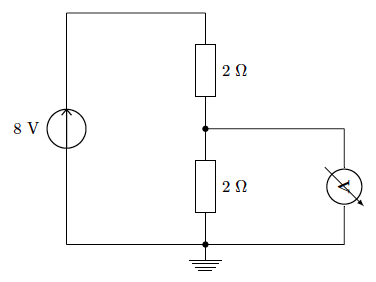
\includegraphics[width=0.55\textwidth]{laborator_01/figuri/5_divizor_cu_voltmetru}
	\caption{Divizorul de tensiune -- influen'ta aparatului de m'asur'a.}
	\label{fig:divizor_cu_voltmetru}
\end{figure}

\begin{exercise}
Ce valoare indic'a voltmetrul din Fig. \ref{fig:divizor_cu_voltmetru}, dac'a:
\begin{itemize}
\item[-] voltmetrul este ideal (rezisten't'a intern'a infinit'a)?
\item[-] voltmetrul este real (rezisten't'a intern'a va fi preluat'a din manualul multimetrului)? % \cite{multimeter_manual})?
\end{itemize}
\end{exercise}


\subsection*{Validare}

Validarea reprezint'a o etap'a extrem de important'a 'in modelare, ea confirm\^and faptul c'a simul'arile 'si experimentele au fost realizate corect. 'In aceast'a etap'a se compar'a rezultatele experimentale cu valorile analitice/simulate. 

\begin{retine}Validarea rezultatelor experimentale
Valoarea analitic'a/simulat'a $\pm$ eroarea ei trebuie s'a se afle 'in intervalul [valoare m'asurat'a -- toleran't'a, valoare m'asurat'a + toleran't'a].
\end{retine}

Pentru ca aceast'a compara'tie s'a fie relevant'a, valorile trebuie s'a aib'a acela'si num'ar de cifre semnificative. Num'arul de cifre semnificative este num'arul de cifre care sunt cunoscute cu certitudine pentru o anumit'a valoare. 

\begin{retine}
Num'arul de cifre semnificative nu este doar num'arul de cifre de dup'a virgul'a (zecimale exacte), ci num'arul total de cifre relevante! \\ 
Valoarea $2.34$ are trei cifre semnficative, 'si dou'a zecimale exacte.
\end{retine}

Num'arul $zero$ trebuie tratat special 'in raportarea cifrelor semnificative. Zerourile de dinaintea primei cifre diferite de zero nu sunt semnificative, f'ar'a s'a conteze unde este virgula (ele indic'a doar ordinul cifrelor urm'atoare 'si pot fi 'intotdeauna eliminate folosind un factor adecvat $10^k$, adic'a mut\^and virgula la dreapta). Zerourile de dup'a virgul'a sunt semnificative, 'in timp ce zerourile de dinainte de virgul'a pot fi semnificative sau nu.
 
\begin{example} Urm'atoarele valori au dou'a cifre semnificative:
$34$, $3.4$, $0.34$, $0.0034$, $3.4\cdot 10^{-4}$ 
\end{example}

\begin{example} Urm'atoarele valori au trei cifre semnificative:
$345$, $3.45$, $0.345$, $0.00345$, $3.45\cdot 10^{-4}$, $3.40$, $0.0340$, $3.40\cdot 10^{-7}$, $3.04$ , $0.000340$
\end{example}

\begin{retine}
'In raportarea unui num'ar 'intreg poate fi neclar c\^ate cifre semnificative sunt folosite. \\
Num'arul $450$ poate fi scris cu dou'a zecimale exacte: $4.5\cdot 10^2$ sau cu trei zecimale exacte: $4.50\cdot 10^2$, dar scrierea $450$ este ambigu'a din acest punct de vedere.
\end{retine}

%\textcolor{red}{$3.4\cdot 10^2$ are doua cifre semnificative ?!}

Modul de raportare a rezultatelor experimentale se face urm\^and anumite reguli.
% (mai multe detalii 'in \cite{cifre_semnificative}):

\begin{enumerate}
\item Erorile absolute ale valorilor determinate experimental nu ar trebui raportate cu mai mult de dou'a cifre semnificative.
\item O valoare 'si marginea erorii absolute asociat'a se raporteaz'a cu exact acela'si num'ar de zecimale exacte (num'ar de cifre dup'a virgul'a).
\begin{example}
Scrierea $2.4\mathrm{~V}\pm 0.16\mathrm{~V}$ implic'a faptul c'a valoarea se afl'a 'in intervalul $2.24\mathrm{~V} - 2.56\mathrm{~V}$. Dar aparatul poate m'asura valori cu o singu'ra zecimal'a exact'a, deci modul corect de raportare este $2.4\mathrm{~V}\pm 0.2\mathrm{~V}$.
\end{example}

\item At\^at valorile m'asurate c\^at 'si erorile absolute corespunz'atoare trebuie s'a aib'a aceea'si unitate de m'asur'a.
\item Raportarea trebuie s'a fie consistent'a 'in nota'tii: dac'a o valoare masurat'a este scris'a 'stiin'tific ($2.3\cdot 10^2$) atunci 'si eroarea absolut'a va fi scris'a tot 'stiin'tific.
\item La efectuarea de opera'tii elementare, rezultatul nu va avea mai multe cifre semnificative dec\^at operandul cu cele mai pu'tine cifre semnificative. Motiva'tia st'a 'in faptul c'a rezultatul nu poate fi mai precis dec\^at valoarea de intrare cea mai pu'tin precis'a. Precizia nu poate fi 'imbun'at'a'tit'a prin efectuarea de calcule. Pentru minimizarea erorilor de rotunjire, se pot utiliza mai multe cifre semnificative 'in calculele intermediare 'si se ajusteaz'a cifrele semnificative numai pentru rezultatele finale.
\begin{example}Cifre semnificative 'in opera'tii elementare: \\
$3.5 \cdot 22.3 = 78, \text{ nu } 78.05$; \\
$6.2 / 833 = 0.0074, \text{ nu } 0.007442977$; \\
$42.4 - 41.62 = 0.8$, $4256 - 24.7 = 4231$, $33.8 + 15.63 = 49.4$.
\end{example}
\end{enumerate}   

\begin{exercise}
Exemple de valorile m'asurate raportate:
\begin{itemize}
\item $0.2 \pm 0.321$ \textcolor{red}{(incorect)}
\item $0 \pm 2$ \textcolor{red}{(corect)}
\item $3.14 \pm 0.02$ \textcolor{red}{(corect)}
%\item $120$ \textcolor{red}{(incorect?)}
\item $3.1421 \pm 0.3214$ \textcolor{red}{(incorect)}
\item $(2.34 \pm 0.15)\cdot 10^{-4}$ \textcolor{red}{(corect)}
\item $(2.34 \pm 0.152)\cdot 10^{-4}$ \textcolor{red}{(incorect)}
\item $0.2 \pm 0.3$ \textcolor{red}{(corect)}
\end{itemize}
\end{exercise}

